\pgfplotsset{width=8cm,compat=1.14}
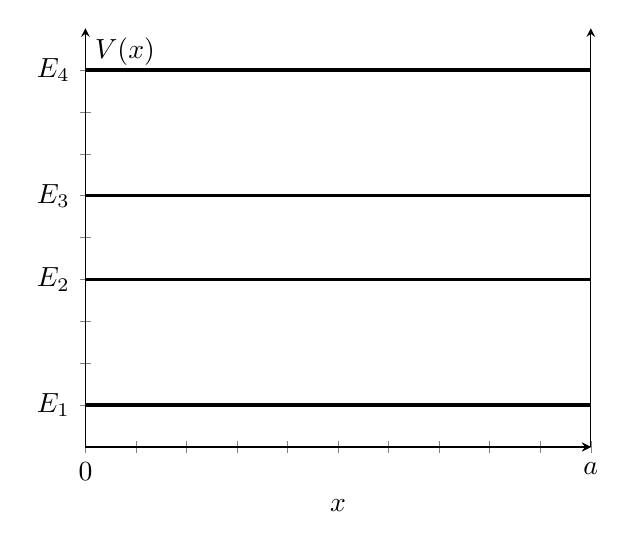
\begin{tikzpicture}
	\begin{axis}
		[
		axis y line=middle,
		axis x line=bottom,
		ymin=0,
		ymax=10,
        ytick={0,1,...,9},
        yticklabels={,$E_1$,,,$E_2$,,$E_3$,,,$E_4$},
		ylabel={$V(x)$},
		xtick={0,1,...,10},
		xticklabels={0,,,,,,,,,,$a$},
		xmin=0,
		xmax=10,
		xlabel={$x$},
		]
        \addplot[black,very thick,samples=200,domain=0:10]{1};
        \addplot[black,very thick,samples=200,domain=0:10]{4};
        \addplot[black,very thick,samples=200,domain=0:10]{6};
        \addplot[black,very thick,samples=200,domain=0:10]{9};
	\end{axis}
	\begin{axis}
		[
		ticks=none,
		xshift=0cm,
		axis lines=middle,
		ymin=0,
		ymax=10,
		xmin=-10,
		xmax=0,
		]
	\end{axis}
\end{tikzpicture}
